Before we start learning the basics of Bayesian filtration, we should extend our knowledge of the Gaussian distribution to the multidimensional case. As mentioned in Section \ref{sec:gauss}, it plays a very important role in object tracking and, in particular, in this work. Formulas and theorems defined in this section are essential for defining and proving the Kalman filter formulas. We will define several properties of multivariate Gaussians required later.

First, we define the multivariate Gaussian distribution with mean vector $\boldsymbol\mu$, covariance matrix $\Sigma$, and evaluated at $\mathbf{x}$ as:

\begin{equation}\label{eq:vec-gauss-def}
    \mathscr{N}\left(\mathbf{x} ; \mathbf\mu, \mathbf\Sigma\right)
    = \frac{1}{\sqrt{(2\pi)^n|\mathbf{\Sigma}|}}\exp\left(-\frac{1}{2}(\mathbf{x}-\boldsymbol{\mu})^\top \mathbf{\Sigma}^{-1} (\mathbf{x}-\boldsymbol{\mu})\right),
\end{equation}

where $n$ is the length of the vector $\mathbf{x}$, and $|\cdot|$ denotes the determinant of a matrix. 

The multivariate Gaussian distribution is a generalization of the univariate Gaussian distribution, where instead of a single mean and variance, we have a mean vector and a covariance matrix that characterizes the correlation between the variables. Note that the exponent contains the expression known as the Mahalanobis distance, which we will encounter throughout this work. It is given by:

\begin{definition}[Mahalanobis distance]\label{def:mahalanobis}
    For vectors $\mathbf x$ and $\mathbf y$ and the symmetrical positive-definite matrix $\mathbf S$, the Mahalanobis distance is defined as:

    \begin{equation}
        d(\mathbf x, \mathbf y) 
        = \sqrt{
            (\mathbf x - \mathbf y)^\intercal
            \mathbf{S}^{-1}
            (\mathbf x - \mathbf y)
        }.
    \end{equation}
\end{definition}

As we will later see, in object tracking, we heavily use conditional probabilities, and in particular, conditioning and marginalization of joint distributions of Gaussian random variables. Thus, we define the following two theorems.

\begin{theorem}[Conditioning on a Gaussian joint distribution]\label{theorem:gauss-cond}
    Let $\mathbf{x}$ and $\mathbf{y}$ be Gaussian random variables with distributions $\mathscr{N}\left(\mathbf{x} ; \mathbf\mu_x, \mathbf\Sigma_{xx}\right)$ and $\mathscr{N}\left(\mathbf{y} ; \mathbf\mu_y, \mathbf\Sigma_{yy}\right)$, respectively. Let their joint probability be given by:

    \begin{equation*}
        p(\mathbf{x}, \mathbf{y}) = \mathscr{N}\left(
            \begin{bmatrix}
                \mathbf{x} \\
                \mathbf{y}
            \end{bmatrix};
            \begin{bmatrix}
                \boldsymbol\mu_x \\
                \boldsymbol\mu_y
            \end{bmatrix},
            \begin{bmatrix}
                \mathbf{\Sigma}_{xx} & \mathbf{\Sigma}_{xy} \\
                \mathbf{\Sigma}_{xy}^\intercal & \mathbf{\Sigma}_{yy}
            \end{bmatrix}
        \right).
    \end{equation*}
    Then the conditional distribution of $\mathbf{x}$ given $\mathbf{y}$ is defined as:
    \begin{equation}\label{eq:gauss-cond}
        p(\mathbf{x}|\mathbf{y}) =
        \mathscr{N}\left(\mathbf{x}; \boldsymbol\mu_{x|y}, \mathbf\Sigma_{x|y}\right),
    \end{equation}
    where
    \begin{align}
        \boldsymbol\mu_{x|y}
        &= \boldsymbol\mu_x + \mathbf{\Sigma}_{xy} \mathbf{\Sigma}_{yy}^{-1}(\mathbf{y} - \boldsymbol\mu_y) \\
        \mathbf\Sigma_{x|y} 
        &= \mathbf\Sigma_{xx} - \mathbf\Sigma_{xy}\mathbf\Sigma_{yy}^{-1}\mathbf\Sigma_{xy}^\intercal.\label{eq:gauss-cond-params}
    \end{align}
\end{theorem}

\begin{theorem}[Marginalization of a Gaussian joint distribution]\label{theorem:gauss-marg}
    Consider the same $\mathbf{x}$, $\mathbf{y}$, $\mathscr{N}\left(\mathbf{x} ; \mathbf\mu_x, \mathbf\Sigma_{xx}\right)$, $\mathscr{N}\left(\mathbf{y} ; \mathbf\mu_y, \mathbf\Sigma_{xx}\right)$ and $p(\mathbf{x}, \mathbf{y})$ given in Theorem \ref{theorem:gauss-cond}. The marginal distribution of $x$ is defined as:

    \begin{equation*}
        p(\mathbf{x}) = \mathscr{N}\left(\mathbf{x} ; \mathbf\mu_x, \mathbf\Sigma_{xx}\right).
    \end{equation*}
\end{theorem}

The proofs for Theorem \ref{theorem:gauss-cond} and Theorem \ref{theorem:gauss-marg} can be found in classical statistical textbooks such as \cite[161--163]{johnsonAppliedMultivariateStatistical2007}.

\subsubsection{Gaussian mixtures}

In multi-target tracking, the posterior density cannot be described in a simple Gaussian distribution. Generally, the posterior distribution can have any form with only assumption that the integral of it sums to one. However, when we are dealing with Gaussian-linear cases, the posterior density is often represented as a mixture of many Gaussian components. A Gaussian mixture is a linear combination of multiple Gaussian distributions and its pdf is expressed in the following way:

\begin{equation}\label{eq:gaussian-mixture}
    p(\mathbf{x}) = \sum_{i=1}^N w_i \mathscr{N}\left(\mathbf{x}; \boldsymbol{\mu}_i, \Sigma_i\right),
\end{equation}

where $N$ is the number of Gaussian components in the mixture, $w_i$ is the weight of the $i$th component, the weights $w_i \geq 0$ sum to one, i.e. $\sum_{i=1}^N w_i = 1$, and each component $\mathscr{N}\left(\mathbf{x}; \boldsymbol{\mu}_i, \Sigma_i\right)$ is a Gaussian distribution with the mean in $\boldsymbol{\mu}_i$ and the covariance matrix $\Sigma_i$. An example of a Gaussian mixture pdf is illustrated in Figure \ref{fig:gaussian-mixture}.

\begin{figure}
\centering
  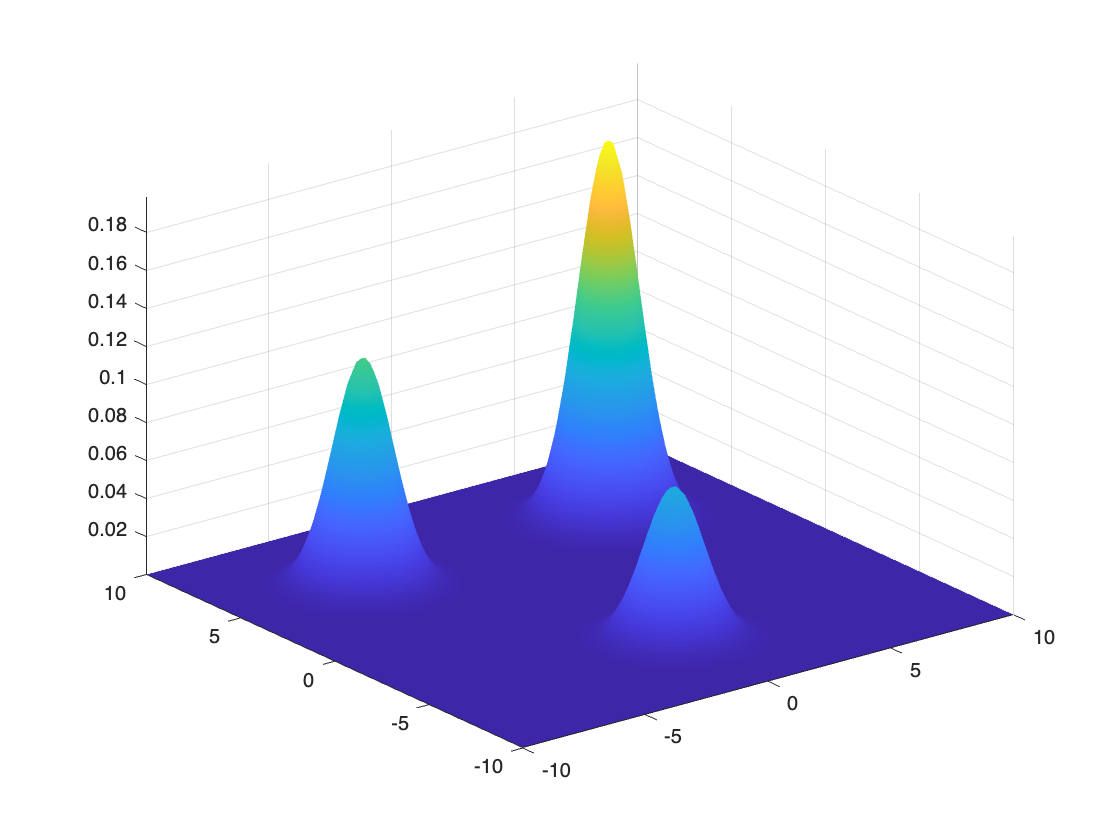
\includegraphics[width=.4\linewidth]{figures/gaussian-mixture.png}
  \caption{An example of a Gaussian mixture with three components. The first component is centered at $[0, -5]^\intercal$ with weight $0.2$, the second component has mean in $[-5, 5]^\intercal$ with weight $0.3$ and the last has mean $[5, 5]^\intercal$ and the weight $0.5$.}
  \label{fig:gaussian-mixture}
\end{figure}

Since the weights sum to one, the Gaussian mixture satisfies the normalization requirement of pdfs and is thus a valid probability density function itself. The weights in the mixture represent the relative importance of the corresponding component. Gaussian mixtures are used to model complex distributions and have several nice mathematical properties as the Gaussian distribution, as we will later see. That is why Gaussian mixtures are widely used to represent posterior distributions in many MTT filters. Moreover, one can easily approximate any distribution with a Gaussian mixture using algorithms such as the Expectation-Maximization algorithm.

A mixture $f(\mathbf{X})$ with $N$ components will have the expected value $\boldsymbol{\hat{\mu}}$ and the covariance $\hat{\Sigma}$ according to the following equations:

\begin{align}
    \boldsymbol{\hat{\mu}} &= \sum_{i=1}^N w_i \boldsymbol{\mu}_i, \\
    \hat{\Sigma} &= \sum_{i=1}^N w_i \Sigma_i + \Tilde{\Sigma},
\end{align}

where the term $\Tilde{\Sigma}$ is called the spread-of-the-innovations and is defined as:

\begin{equation}
    \Tilde{\Sigma}= \sum_{i=1}^N
        w_i (\boldsymbol{\mu}_i - \hat{\boldsymbol{\mu}})
        (\boldsymbol{\mu}_i - \hat{\boldsymbol{\mu}})^\intercal.
\end{equation}

The spread-of-the-innovations quantifies the magnitude of the difference between expectations of individual components.
